%%% In this section, you will describe all of the various artifacts that you will generate and maintain during the project life cycle. Describe the purpose of each item below, how the content will be generated, where it will be stored, how often it will be updated, etc. Replace the default text for each section with your own description. Reword this paragraph as appropriate.

\subsection{Major Documentation Deliverables}

\subsubsection{Project Charter}
The project charter initial draft will be delivered at the end of Sprint 1, on June 25th 2025. It will be maintained and updated at the end of each sprint by a different assigned team member.
**Describe how this document will be maintained and updated (how often, under what circumstances, etc.). When will the initial version be delivered? When will the final version be delivered?

\subsubsection{System Requirements Specification}
**Describe how this document will be maintained and updated (how often, under what circumstances, etc.). When will the initial version be delivered? When will the final version be delivered?

\subsubsection{Architectural Design Specification}
**Describe how this document will be maintained and updated (how often, under what circumstances, etc.). When will the initial version be delivered? When will the final version be delivered?

\subsubsection{Detailed Design Specification}
**Describe how this document will be maintained and updated (how often, under what circumstances, etc.). When will the initial version be delivered? When will the final version be delivered?

\subsection{Recurring Sprint Items}

\subsubsection{Product Backlog}
**How will items be added to the product backlog from the SRS? How will these items be prioritized? Who makes the decision (product owner, group vote, etc.)? What software will be used to maintain and share the product backlog with team members and stakeholders?

\subsubsection{Sprint Planning}
**How will each sprint plan be planned? How many sprints will there be (you need to look at the schedules for this course and previous Senior Design II courses during the appropriate semesters to figure this out).

\subsubsection{Sprint Goal}
**Who decides the sprint goal? How will you involve your customer in this process?

\subsubsection{Sprint Backlog}
**Who decides which product backlog items make their way into the sprint backlog? How will the backlog be maintained (collaboration software, a "scrum board", etc.)?

\subsubsection{Task Breakdown}
**How will individual tasks be assigned from the sprint backlog? Will it be up to each team member to voluntarily claim a task, or will it come from the product owner? How will time spent on tasks be documented?

\subsubsection{Sprint Burn Down Charts}
**Who will be responsible for generating the burn down charts for each sprint? How will they be able to access the total amount of effort expended by each individual team member? What format will the burn down chart use (include an example burn down chart below).

\begin{figure}[h!]
    \centering
    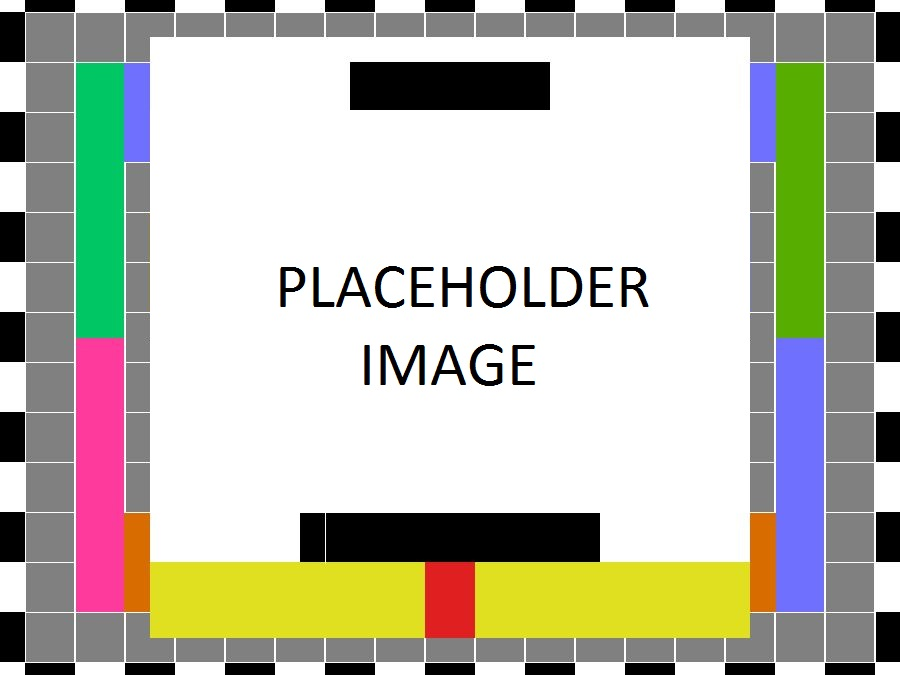
\includegraphics[width=0.5\textwidth]{images/test_image}
    \caption{Example sprint burn down chart}
\end{figure}

\subsubsection{Sprint Retrospective}
**How will the sprint retrospective be handled as a team? When will this discussion happen after each sprint? What will be documented as a group and as individuals, and when will it be due?

\subsubsection{Individual Status Reports}
**What sort of status will be reported by each individual member, and how often will it be reported? What key items will be contained in the report?

\subsubsection{Engineering Notebooks}
**How often will the engineering notebook be updated, at a minimum, by each team member? What is the minimum amount of pages that will be completed for each interval, and how long will that interval be? How will the team keep each member accountable? Who will sign of as a "witness" for each ENB page?

\subsection{Closeout Materials}

\subsubsection{System Prototype}
The final system prototype will include the AR software, printed table markers, and any supporting materials required for proper operation on smartphones/tablets. The prototype will be demonstrated to the sponsor, and to other students, during the final sprint and showcase the systems functionality and educational features. A Prototype Acceptance Test (PAT) will be conducted to confirm the system meets the sponsors requirements. It is not likely for there to be an off-site demonstration, but if necessary, a Field Acceptance Test (FAT) may also be arranged to cofirm performance in the intended use environment. The project will be delivered at project conclusion, along with documentation to support future use.

\subsubsection{Project Poster}
The project poster will summarize the AR Wetlands system, including its goals, technical approach, and educational impact. It will contain sections such as: Executive Summary, Background, Key Requirements, System Design, Implementation and Test Plan, Results, Conclusions, and References. The final dimensions are still to be determined, but will likely be 4'x3'. It will be delivered by the conclusion of Senior Design 2, approximately December 5th 2025.

\subsubsection{Web Page}
The project web page will serve as a public-facing summary of the AR Wetlands Project, highlighting its purpose, features, and key technical details. It will include an overview of the system, authorized sponsor information, team members, project poster, demo video, and links to relevant authorized documentation. It will be delivered at the conclusion of Senior Design 2, around December 3rd, 2025, but will be worked on and updated throughout project.

\subsubsection{Demo Video}
Our demo video will cover system functionality and use, such as startup, how users interact with the AR table, trigger educational content and animations. It will be approximately 4-7 minutes long. B-reel footage of shots of the table and app interface will be included for future video cuts.

\subsubsection{Source Code}
We will be using GitHub for version control and maintenance. The sponsor will receive the source code at the conclusion of the project directly. Licensing and open source is still to be determined, but will be included in the readme file. A license file will be included in the repository root.

\subsubsection{Source Code Documentation}
Industry standards will be employed for documentation. Tools such as Doxygen will be used. Final documentation will be provided in pdf or html.

%\subsubsection{Hardware Schematics}
%**Will you be creating printed circuit boards (PCBs) or wiring components together? If so, list each applicable schematic and what sort of data it will contain (PCB layout, wiring diagram, etc.). If your project is purely software, omit this section.

%\subsubsection{CAD files}
%**Will the project involve any mechanical design, such as 3D printed or laser-cut parts? If so, what software will you use to generate the files and what file formats will you provide in your closeout materials (STL, STEP, OBJ, etc.). If your project is purely software, omit this section.

\subsubsection{Installation Scripts}
**How will the customer deploy software to new installations? Will you provide installation scripts, install programs, or any other tools to improve the process? Will there be multiple scripts provided (perhaps separate scripts for the graphical front end and back end server software)? 

\subsubsection{User Manual}
A digital user manual and setup video will be provided at the conclusion of the project.
